% Multi-panel figure: iterations to match the unrolled networks, exp2_try3_210x300.
% Generated by plot_compute_matched_rf.py --run exp2_try3_210x300. Requires \usepackage{graphicx}
% and \usepackage{subcaption}. Paths are relative to the repo root (Figs/...);
% adjust \graphicspath or the paths below to match the Overleaf project.
% Include with: % Multi-panel figure: iterations to match the unrolled networks, exp2_try3_210x300.
% Generated by plot_compute_matched_rf.py --run exp2_try3_210x300. Requires \usepackage{graphicx}
% and \usepackage{subcaption}. Paths are relative to the repo root (Figs/...);
% adjust \graphicspath or the paths below to match the Overleaf project.
% Include with: % Multi-panel figure: iterations to match the unrolled networks, exp2_try3_210x300.
% Generated by plot_compute_matched_rf.py --run exp2_try3_210x300. Requires \usepackage{graphicx}
% and \usepackage{subcaption}. Paths are relative to the repo root (Figs/...);
% adjust \graphicspath or the paths below to match the Overleaf project.
% Include with: % Multi-panel figure: iterations to match the unrolled networks, exp2_try3_210x300.
% Generated by plot_compute_matched_rf.py --run exp2_try3_210x300. Requires \usepackage{graphicx}
% and \usepackage{subcaption}. Paths are relative to the repo root (Figs/...);
% adjust \graphicspath or the paths below to match the Overleaf project.
% Include with: \input{Figs/multifigure/iterations_to_match_exp2_try3_210x300_figure}
\begin{figure}[htbp]
\centering
\begin{subfigure}[t]{0.48\linewidth}
  \centering
  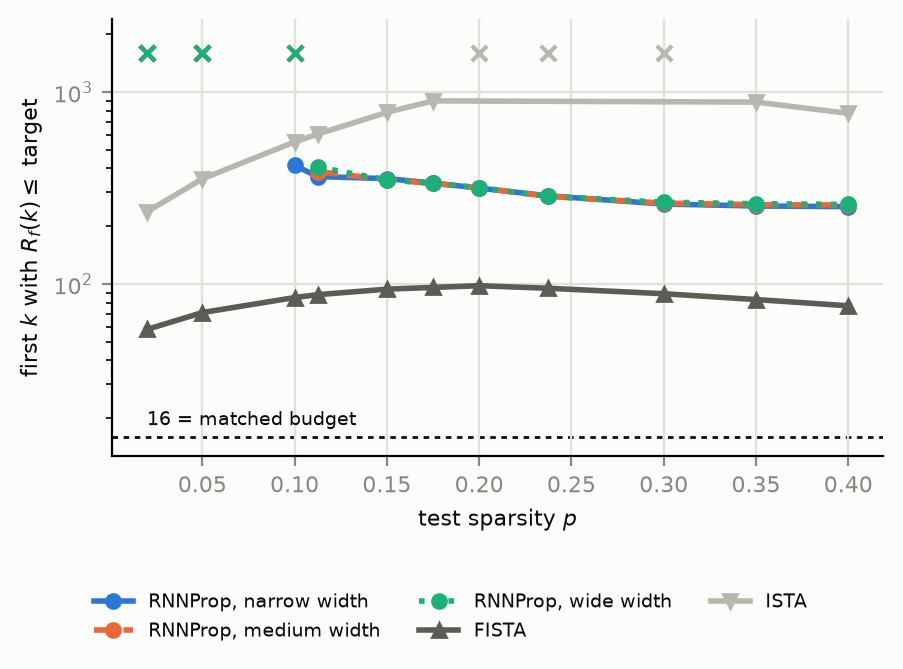
\includegraphics[width=\linewidth]{Figs/exp2_try3_210x300/iterations_to_match_exp2_try3_210x300_lista.png}
  \caption{Iterations to reach LISTA's 16-layer $R_f$}
  \label{fig:iterations-to-match-exp2-try3-210x300-lista}
\end{subfigure}\hfill
\begin{subfigure}[t]{0.48\linewidth}
  \centering
  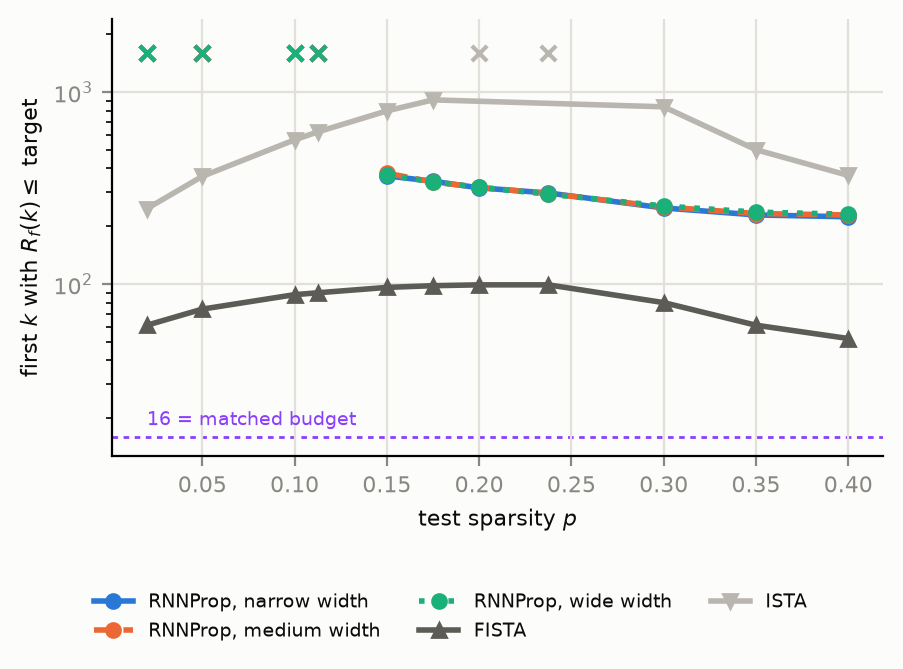
\includegraphics[width=\linewidth]{Figs/exp2_try3_210x300/iterations_to_match_exp2_try3_210x300_alista.png}
  \caption{Iterations to reach ALISTA's 16-layer $R_f$}
  \label{fig:iterations-to-match-exp2-try3-210x300-alista}
\end{subfigure}
\caption{Iteration budget needed to match the 16-layer unrolled networks on the modified relative loss $R_f$ (Eq.~10), $(m,n) = (210, 300)$, noiseless, centred widths. For each test sparsity $p$, the first iteration $k$ at which a method's $R_f(k)$ falls to or below the 16-layer LISTA (left) or ALISTA (right) value (median over seeds and over the three training widths); RNNProp (median over 5 seeds; one curve per training width), and textbook ISTA and FISTA from the same shared $x_0$ (median over seeds). The dotted line marks the matched budget of 16 iterations; a cross above the 1000-iteration line means the target was never reached within the evaluation horizon. Iteration-matched is not compute-matched: one learned step is an LSTM forward pass per coordinate, one ISTA/FISTA step a matrix product.}
\label{fig:iterations-to-match-exp2-try3-210x300}
\end{figure}

\begin{figure}[htbp]
\centering
\begin{subfigure}[t]{0.48\linewidth}
  \centering
  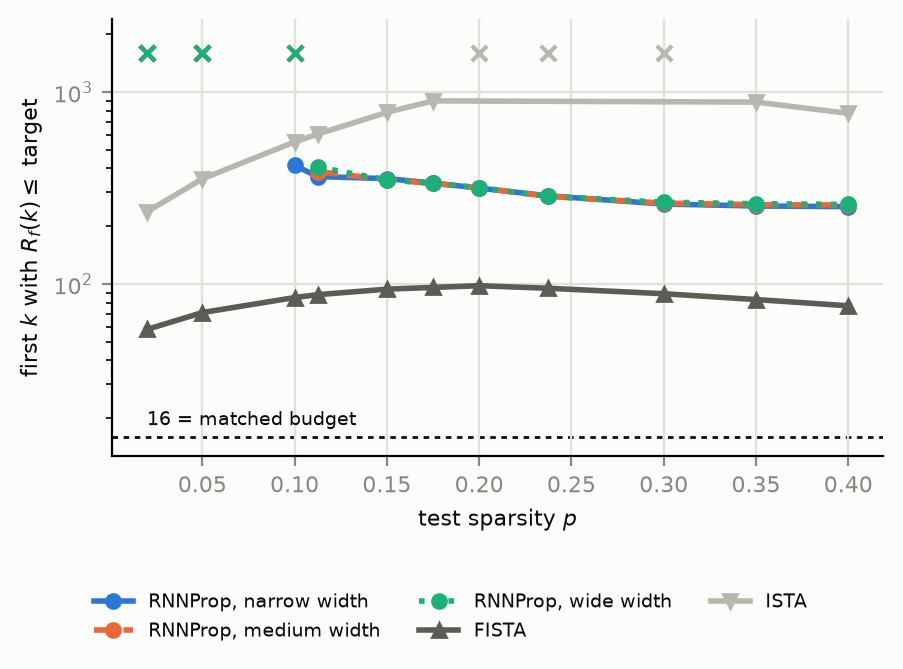
\includegraphics[width=\linewidth]{Figs/exp2_try3_210x300/iterations_to_match_exp2_try3_210x300_lista.png}
  \caption{Iterations to reach LISTA's 16-layer $R_f$}
  \label{fig:iterations-to-match-exp2-try3-210x300-lista}
\end{subfigure}\hfill
\begin{subfigure}[t]{0.48\linewidth}
  \centering
  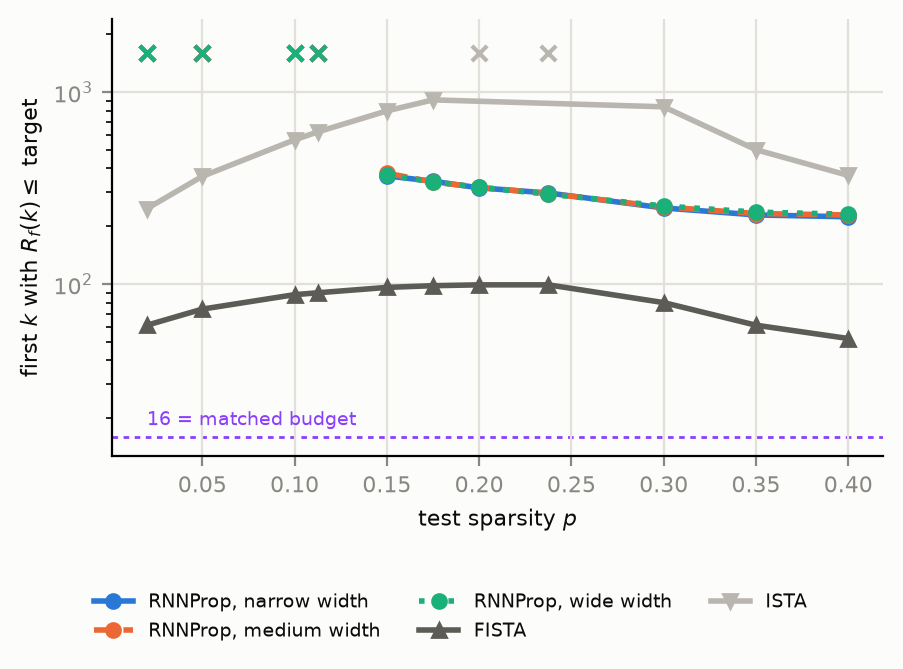
\includegraphics[width=\linewidth]{Figs/exp2_try3_210x300/iterations_to_match_exp2_try3_210x300_alista.png}
  \caption{Iterations to reach ALISTA's 16-layer $R_f$}
  \label{fig:iterations-to-match-exp2-try3-210x300-alista}
\end{subfigure}
\caption{Iteration budget needed to match the 16-layer unrolled networks on the modified relative loss $R_f$ (Eq.~10), $(m,n) = (210, 300)$, noiseless, centred widths. For each test sparsity $p$, the first iteration $k$ at which a method's $R_f(k)$ falls to or below the 16-layer LISTA (left) or ALISTA (right) value (median over seeds and over the three training widths); RNNProp (median over 5 seeds; one curve per training width), and textbook ISTA and FISTA from the same shared $x_0$ (median over seeds). The dotted line marks the matched budget of 16 iterations; a cross above the 1000-iteration line means the target was never reached within the evaluation horizon. Iteration-matched is not compute-matched: one learned step is an LSTM forward pass per coordinate, one ISTA/FISTA step a matrix product.}
\label{fig:iterations-to-match-exp2-try3-210x300}
\end{figure}

\begin{figure}[htbp]
\centering
\begin{subfigure}[t]{0.48\linewidth}
  \centering
  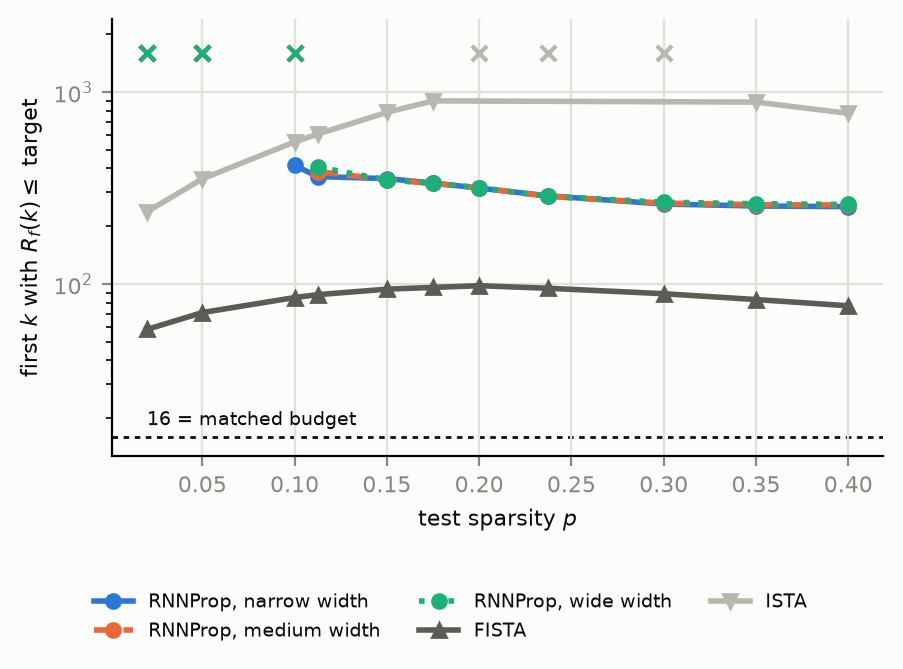
\includegraphics[width=\linewidth]{Figs/exp2_try3_210x300/iterations_to_match_exp2_try3_210x300_lista.png}
  \caption{Iterations to reach LISTA's 16-layer $R_f$}
  \label{fig:iterations-to-match-exp2-try3-210x300-lista}
\end{subfigure}\hfill
\begin{subfigure}[t]{0.48\linewidth}
  \centering
  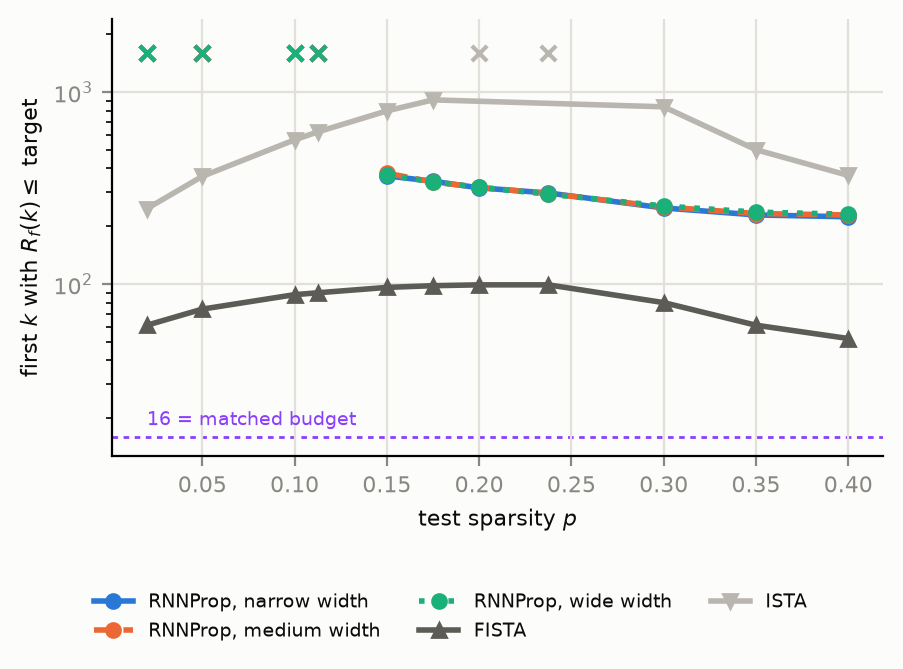
\includegraphics[width=\linewidth]{Figs/exp2_try3_210x300/iterations_to_match_exp2_try3_210x300_alista.png}
  \caption{Iterations to reach ALISTA's 16-layer $R_f$}
  \label{fig:iterations-to-match-exp2-try3-210x300-alista}
\end{subfigure}
\caption{Iteration budget needed to match the 16-layer unrolled networks on the modified relative loss $R_f$ (Eq.~10), $(m,n) = (210, 300)$, noiseless, centred widths. For each test sparsity $p$, the first iteration $k$ at which a method's $R_f(k)$ falls to or below the 16-layer LISTA (left) or ALISTA (right) value (median over seeds and over the three training widths); RNNProp (median over 5 seeds; one curve per training width), and textbook ISTA and FISTA from the same shared $x_0$ (median over seeds). The dotted line marks the matched budget of 16 iterations; a cross above the 1000-iteration line means the target was never reached within the evaluation horizon. Iteration-matched is not compute-matched: one learned step is an LSTM forward pass per coordinate, one ISTA/FISTA step a matrix product.}
\label{fig:iterations-to-match-exp2-try3-210x300}
\end{figure}

\begin{figure}[htbp]
\centering
\begin{subfigure}[t]{0.48\linewidth}
  \centering
  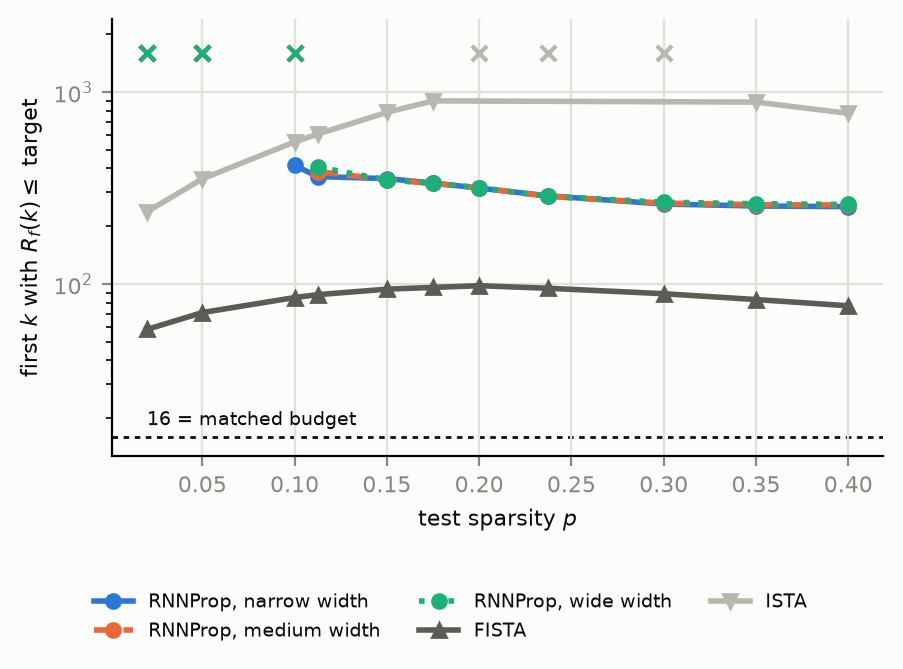
\includegraphics[width=\linewidth]{Figs/exp2_try3_210x300/iterations_to_match_exp2_try3_210x300_lista.png}
  \caption{Iterations to reach LISTA's 16-layer $R_f$}
  \label{fig:iterations-to-match-exp2-try3-210x300-lista}
\end{subfigure}\hfill
\begin{subfigure}[t]{0.48\linewidth}
  \centering
  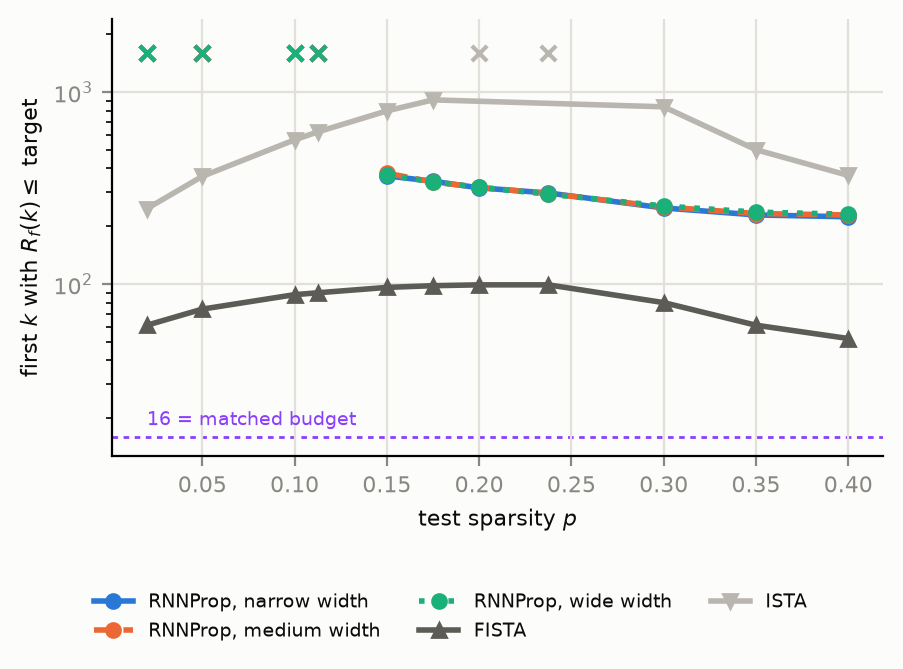
\includegraphics[width=\linewidth]{Figs/exp2_try3_210x300/iterations_to_match_exp2_try3_210x300_alista.png}
  \caption{Iterations to reach ALISTA's 16-layer $R_f$}
  \label{fig:iterations-to-match-exp2-try3-210x300-alista}
\end{subfigure}
\caption{Iteration budget needed to match the 16-layer unrolled networks on the modified relative loss $R_f$ (Eq.~10), $(m,n) = (210, 300)$, noiseless, centred widths. For each test sparsity $p$, the first iteration $k$ at which a method's $R_f(k)$ falls to or below the 16-layer LISTA (left) or ALISTA (right) value (median over seeds and over the three training widths); RNNProp (median over 5 seeds; one curve per training width), and textbook ISTA and FISTA from the same shared $x_0$ (median over seeds). The dotted line marks the matched budget of 16 iterations; a cross above the 1000-iteration line means the target was never reached within the evaluation horizon. Iteration-matched is not compute-matched: one learned step is an LSTM forward pass per coordinate, one ISTA/FISTA step a matrix product.}
\label{fig:iterations-to-match-exp2-try3-210x300}
\end{figure}
